\subsection{Analisi}

Il periodo di analisi comincia il 2018-11-15 e si conclude il 2019-01-14. L'inizio coincide con la data di formazione del gruppo e l'avvio dei primi lavori. La conclusione coincide con la scadenza scelta per presentare la documentazione d'ingresso al progetto.

\subsubsection{Incrementi}
Durante il periodo sopra descritto vengono effettuati 6 incrementi, ognuno per un'attività principale.\\
Le attività principali sono:
\begin{itemize}

	\item \textbf{\gl{Studio di Fattibilità}:} questa attività consiste nell'analisi dei vari capitolati proposti ed è importante per scegliere con attenzione il capitolato da svolgere. Viene redatto il documento di supporto Studio di fattibilità contenente l'analisi effettuata per ogni capitolato. Questa attività va obbligatoriamente svolta prima del'\gl{Analisi dei Requisiti} in quanto bisogna essere certi del capitolato che si intende svolgere;

	\item \textbf{Norme di Progetto:} in questa prima attività l'\emph{Amministratore} stabilisce tutte le norme che i membri del gruppo 7DOS devono rispettare fino alla conclusione del progetto. Viene redatto il documento di supporto Norme di Progetto che contiene tutte le norme stabilite. Questa attività è di massima importanza considerando che le Norme di Progetto stabiliscono anche le norme e gli strumenti utilizzati per la stesura dei documenti;

	\item \textbf{Analisi dei Requisiti:} partendo dalla bozza di analisi ad alto livello redatta durante lo Studio di Fattibilità si genera un'analisi approfondita. Durante questa analisi si ricavano e analizzano tutti i requisiti del capitolato scelto e si riportano nel documento Analisi dei Requisiti;

	\item \textbf{Piano di Qualifica:} in questa attività l'Analista insieme al Responsabile di Progetto individua i metodi per garantire la \gl{qualità di prodotto}. Una volta individuati vengono redatti all'interno del documento \textit{Piano di qualifica};

	\item \textbf{Piano di Progetto:} il \emph{Responsabile di Progetto}, partendo dalle date ufficiali e dalle relative scadenze, redige il Piano di Progetto così da organizzare le attività del gruppo. Si analizzano anche i rischi nei quali il gruppo può incombere e le relative soluzioni. Si suddividono anche le risorse disponili per l'intera durata del progetto;

	\item \textbf{Glossario:} in questa attività si individuano tutti i termini considerati poco chiari o ambigui e li si aggiungono nel documento contenente il Glossario;
	
	\item \textbf{Lettera di presentazione:} documento di presentazione del gruppo per la partecipazione alla gara d'appalto per il capitolato.

\end{itemize}

\subsubsection{Analisi - Gantt delle attività}

\begin{figure} [H]
	\centering
	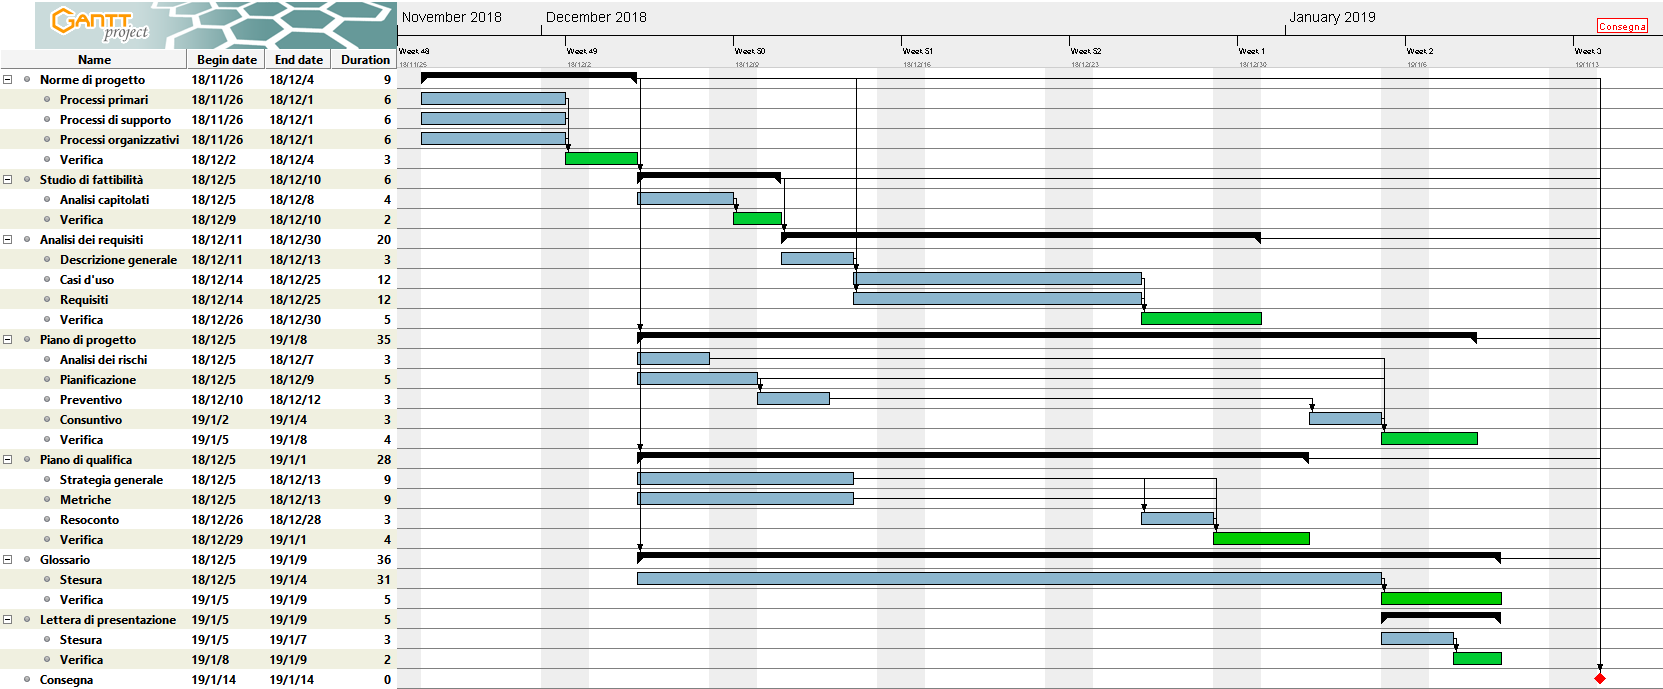
\includegraphics[scale=0.3]{Res/Gantt/Analisi}
	\caption{Figura 4.1: Diagramma di Gantt del periodo "Analisi"}\label{}
\end{figure}

\pagebreak
